\section{Background}
\label{sec:vibvoice_background}
This section introduces EarSense, an open-source wearable platform with a sensing setup similar to current commercial HMWs (Section~\ref{sec:vibvoice_EarSense}). It then analyzes bone-conducted vibration and audio signals recorded by EarSense under several settings (Section~\ref{sec:vibvoice_measurement}). Finally, it summarizes the VibVoice design (Section~\ref{sec:vibvoice_overview}) and introduces the Bone Conduction Function and multimodal network (Sections~\ref{sec:vibvoice_bcf} and~\ref{sec:vibvoice_network}).


\subsection{EarSense: An Open Source Data Collection Platform for HMWs}
\label{sec:vibvoice_EarSense}

Most commercial HMWs do not provide APIs to collect raw acceleration data. Apple provides APIs~\citep{CMHeadph3:online} for collecting AirPods motion data at $100\,\text{Hz}$, but this sampling rate is too low for speech-related vibration and does not fully use the commercial IMU.
We therefore develop a sensing platform that can: a) collect acceleration and acoustic data synchronously at a sample rate suitable for speech information; b) maintain contact with the user's head in a manner similar to HMWs; and c) remain compatible with existing commercial devices.
\begin{figure}
  \begin{subfigure}{.64\columnwidth}
    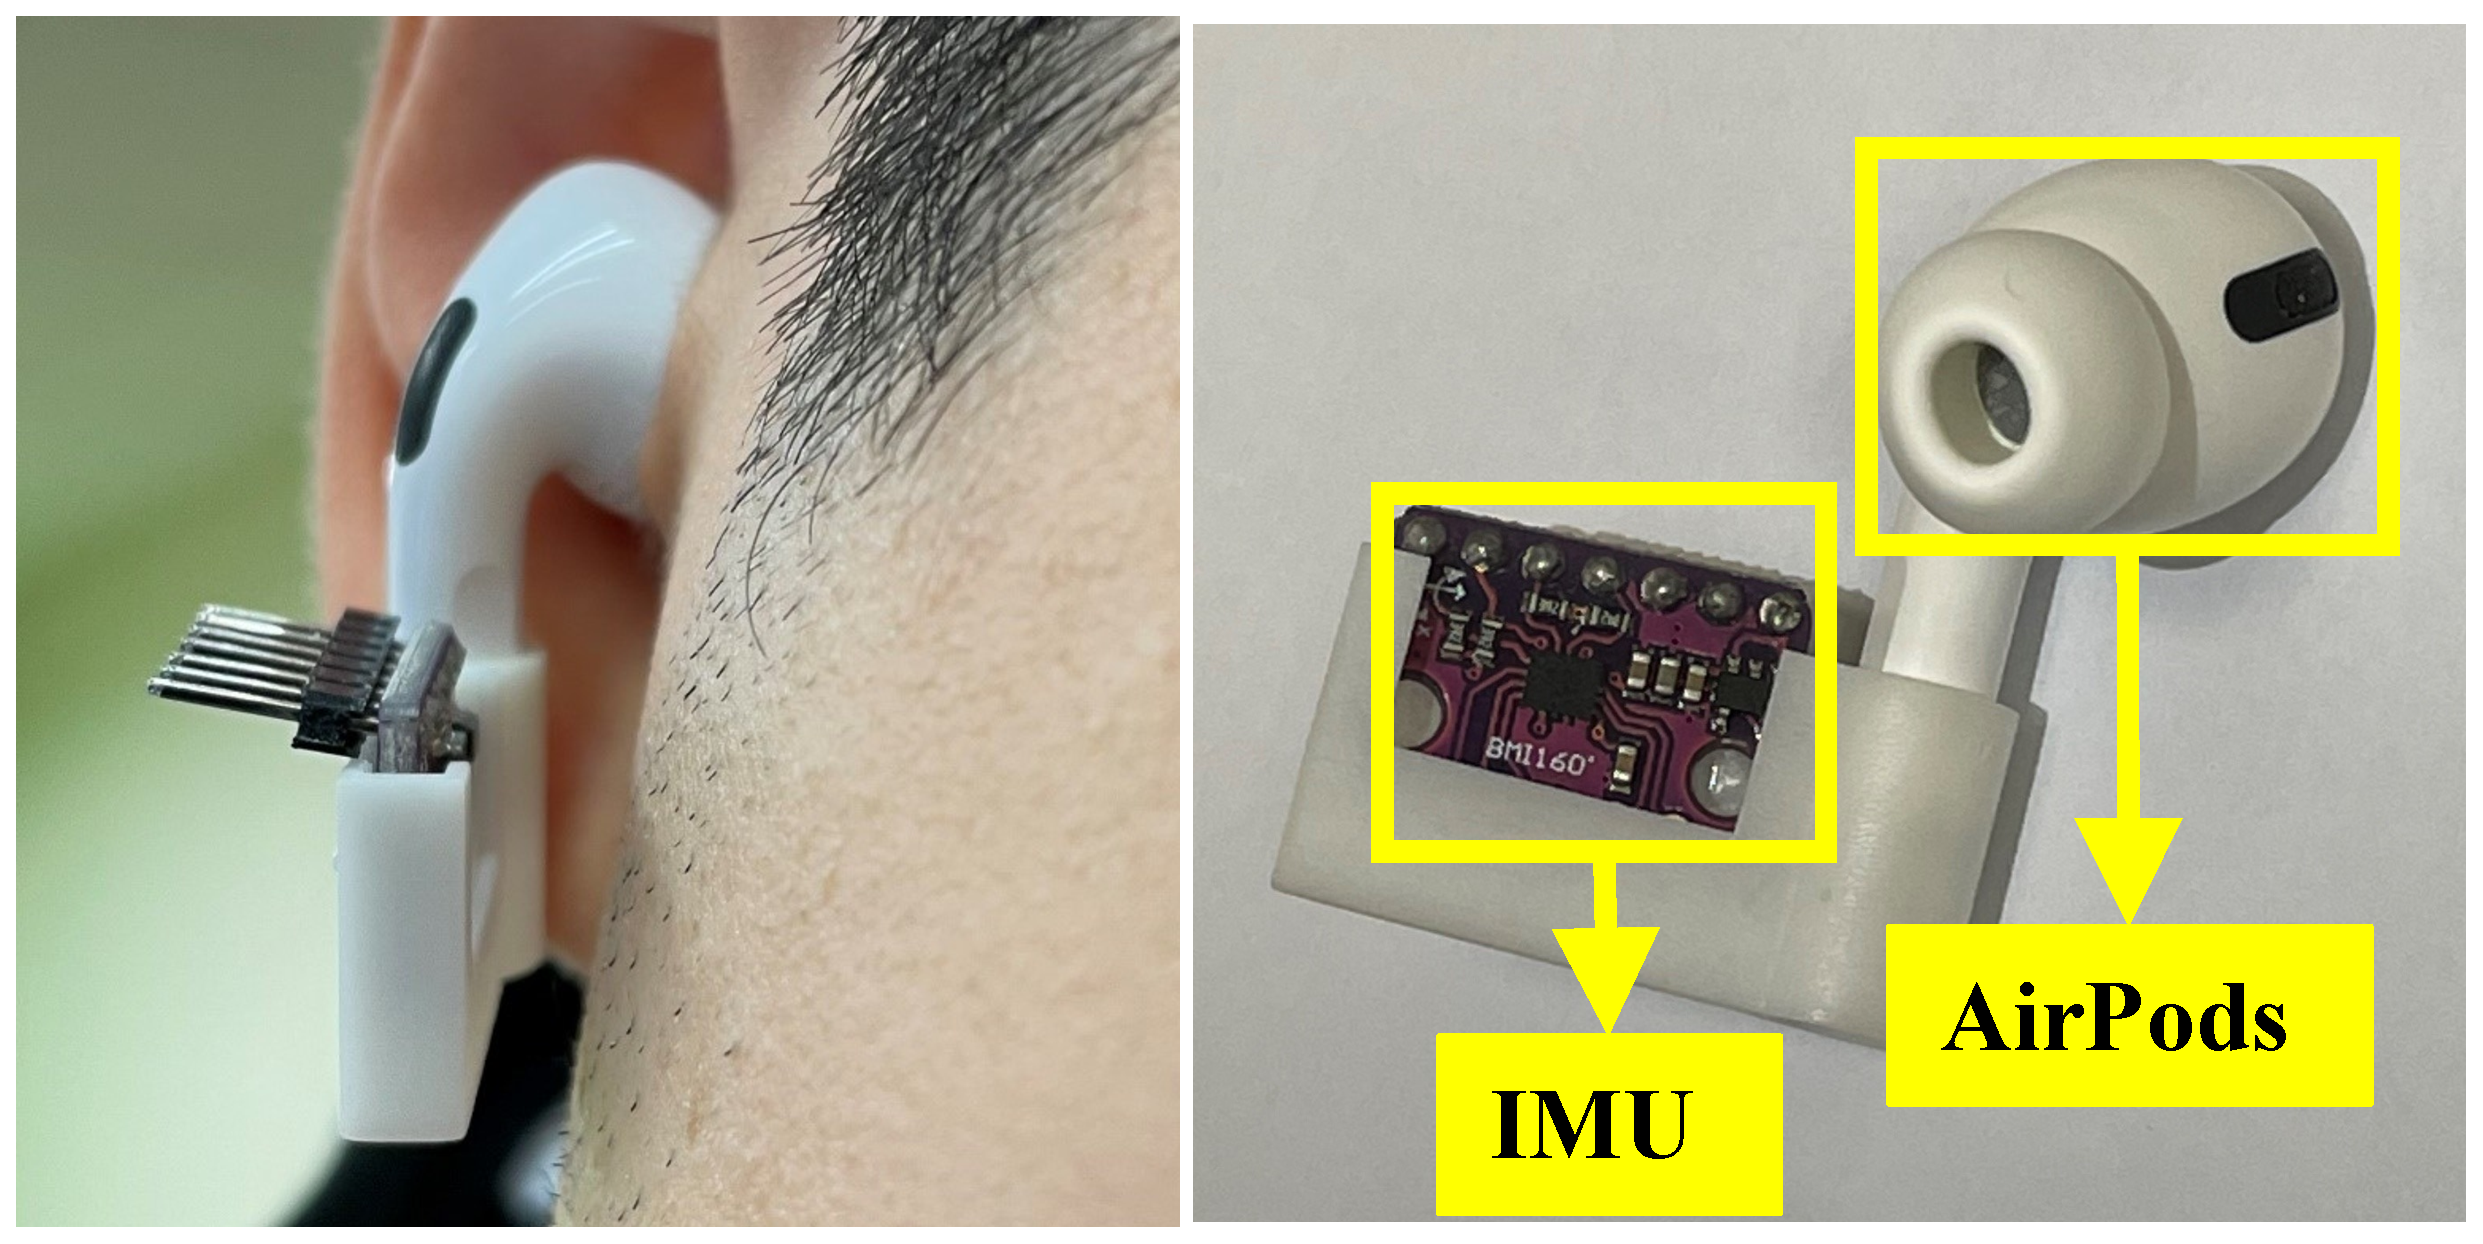
\includegraphics[width=\textwidth]{chapters/vibvoice/figure/earsense.eps}
    \caption{\emph{EarSense} with an Airpods Pro.}
    \label{fig:vibvoice_earsense-head}
  \end{subfigure}
  \begin{subfigure}{0.35\columnwidth}
    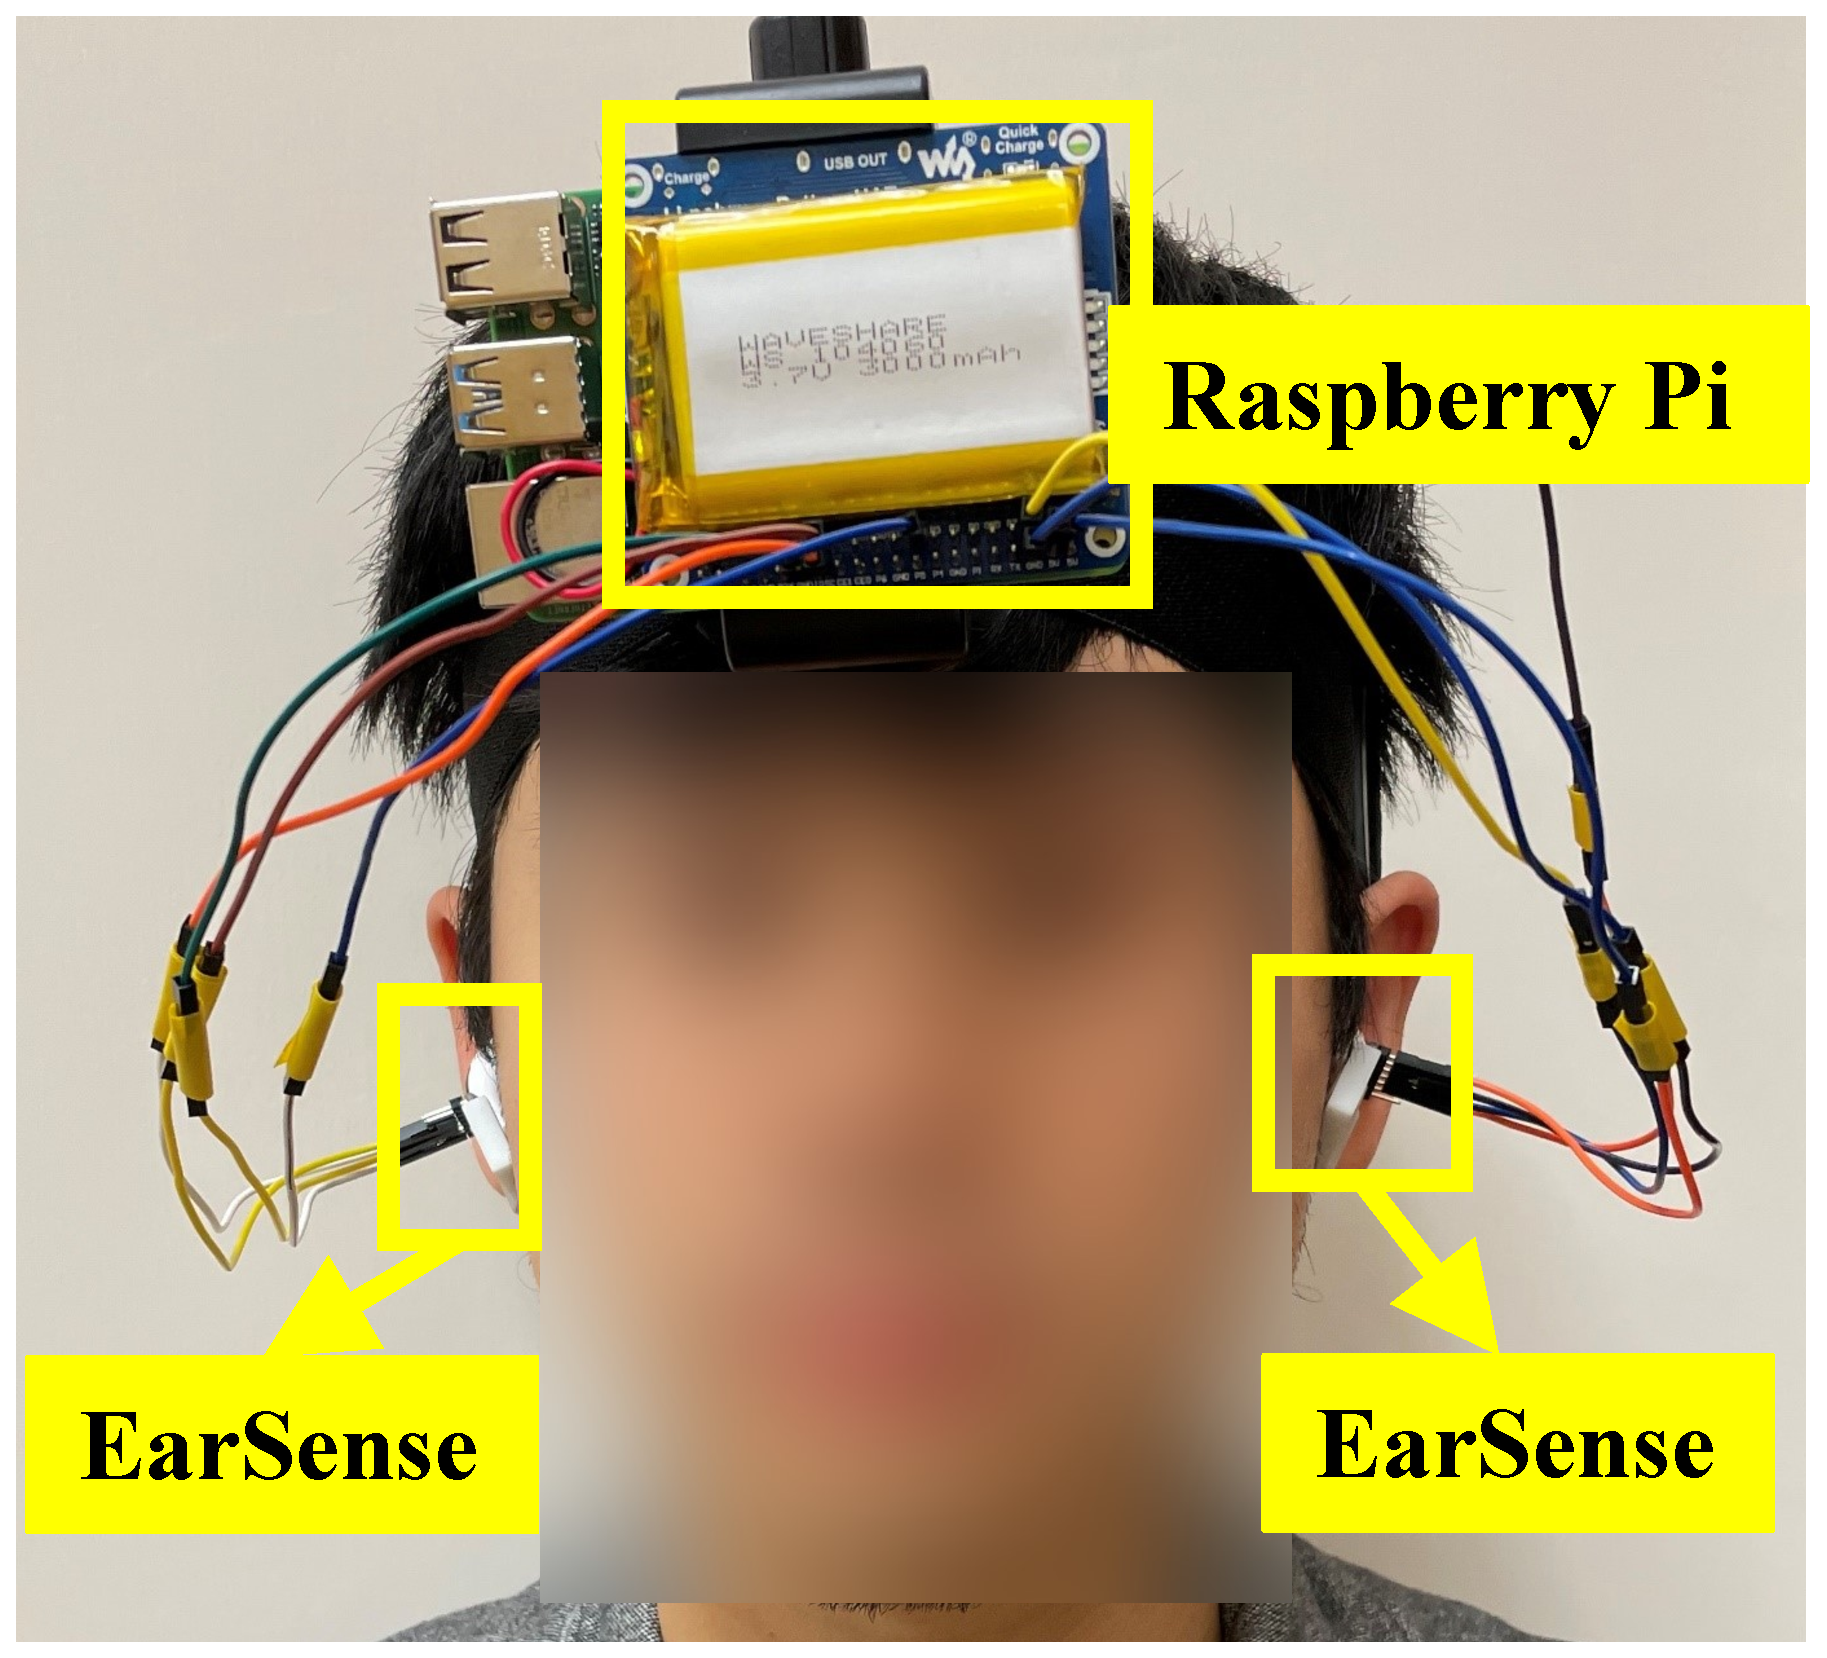
\includegraphics[width=\textwidth]{chapters/vibvoice/figure/people.eps}
    \caption{Test Setup.}
    \label{fig:vibvoice_earsense-people}
  \end{subfigure}
  \caption{\emph{EarSense} is an open-sourced data collector attachable to commercial HMWs for vibration sensing.}
  \label{fig:vibvoice_earsense}
\end{figure}

Fig. \ref{fig:vibvoice_earsense} shows the prototype of \textit{EarSense}  \citep{dataset}, a new open-sourced sensing platform that equips a 3D-printed enclosure with an IMU sensor (i.e., Bosch BMI-160 \citep{Inertial63:online}) inserted. EarSense has a flexible design to make it attachable to any commercial HMW device (e.g., AirPods Pro). EarSense captures the same vibration as the testing HMW and has no direct contact with the user's head (shown in Fig. \ref{fig:vibvoice_earsense-head}).
We connect two EarSenses to a Raspberry Pi (RPi) with a battery for data collection.
Fig. \ref{fig:vibvoice_earsense-people} shows a volunteer wearing the device on the head to avoid excessive vibrations caused by the connecting wires.
A Python script on the RPi controls the EarSense devices through the I2C protocol and stores the data for offline processing.
We only use the three-axis accelerometer provided by the IMU chip because the gyroscope and magnetometer are less related to the vibration.
The default sample rates of the microphone and accelerometer are $16\,\text{kHz}$ and $1.6\,\text{kHz}$, respectively. Since commercial earphones such as AirPods Pro do not support two-channel audio recording through public APIs, EarSense records audio in a mono channel.
We apply L2-Norm to the spectrograms of three-axis acceleration to extract the vibration intensity and avoid the impact of wearing position and user's motion.

\subsection{Measurements of Bone-Conducted Vibrations}
\label{sec:vibvoice_measurement}
We measure the difference between audio and bone-conducted vibrations with EarSense under various settings, i.e., the noises caused by the competing speaker and user motion. In each experiment, we ask a volunteer to wear Apple AirPods Pro with EarSense attached (shown in Fig. \ref{fig:vibvoice_earsense-people}) in a meeting room with the size of $10~\text{m}^2$. 
\begin{figure}
    \begin{subfigure}{0.46\columnwidth}
        \centering
        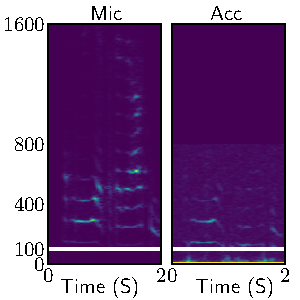
\includegraphics[width=1\textwidth]{chapters/vibvoice/figure/clean.pdf}
        \caption{The user is talking with no noise.}
        \label{fig:vibvoice_nospeaker}
        \end{subfigure}
        \hspace{.5em}
    \begin{subfigure}{0.46\columnwidth}
        \centering
        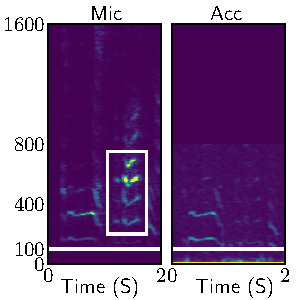
\includegraphics[width=1\textwidth]{chapters/vibvoice/figure/noise.pdf}
        \caption{The user is talking with a competing speaker.}
        \label{fig:vibvoice_speaker}
         \end{subfigure}
    \caption{Impact of the competing speaker.}
    \label{fig:vibvoice_competing-speaker}
\end{figure}

\noindent\textbf{Competing speaker.}
First, we ask the user to sit in the meeting room and speak while a loudspeaker is playing a pre-recording speech one meter from the user as the competing speaker. Note that the competing speaker is one of the most challenging environmental noises for HMWs since its spectrum is similar to the speech's, making it indistinguishable from the noise suppression algorithms. 
We set the volume of the competing speaker to be similar to the user, in which SNR is 3 dB. It is difficult to separate the two sources according to volume since the two speeches are mixed.
Fig. \ref{fig:vibvoice_nospeaker} and Fig. \ref{fig:vibvoice_speaker} show the spectrograms of microphone audio and acceleration when the environment is quiet or contains a competing speaker when the user is talking, respectively.
Note that we only show the spectrogram up to $1.6\,\text{kHz}$ since there is slim energy in the frequency bands higher than $1.6\,\text{kHz}$ of the microphone, and the accelerometer can only sense the signal with a frequency band of $800\,\text{Hz}$.
The spectrograms show that acceleration has lower signal energy than microphone audio since acoustic vibration attenuates during bone conduction, especially for high-frequency vibrations. Compared with the silent environment, the audio spectrogram of microphone audio with a competing speaker shows strong distortions, as highlighted with the white box in Fig. \ref{fig:vibvoice_speaker}. However, the accelerometer spectrograms do not show this phenomenon because the competing speaker cannot produce bone-conducted vibrations.
In summary, the accelerometer receives the user's voice through bone conduction only, excluding environmental sounds over the air, which is ideal for speech enhancement.

\noindent\textbf{User motion.}
We also measure the noises caused by the user's motion. We ask the volunteer to walk while talking. Fig. \ref{fig:vibvoice_walk} shows that walking causes low-frequency noises in the acceleration. The green boxes show the zoom-in result of the signals below $100\,\text{Hz}$. We can observe clear periodic fluctuations in low frequency (i.e., $< 50\,\text{Hz}$), which are caused by the steps of the volunteer.
In summary, the user's motion only affects the acceleration at lower frequencies, which does not affect our speech enhancement.
In addition, we observe slight low-frequency fluctuation in acceleration in Fig. \ref{fig:vibvoice_competing-speaker}, although the volunteer is asked to stand still in this experiment. Since most of the human speech is above $85~\text{Hz}$ \citep{Voicefre75:online}, the removal of audio in low frequency (i.e., the white horizontal lines in Fig. \ref{fig:vibvoice_competing-speaker}) can effectively reduce the interference caused by human motion.

\begin{figure}
\begin{minipage}[t]{0.46\columnwidth}
     \centering
        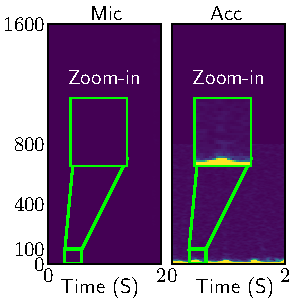
\includegraphics[width=1\textwidth]{chapters/vibvoice/figure/notalk.pdf}
        \caption{Spectrograms of microphone and acceleration when the user is walking.}
        \label{fig:vibvoice_walk}
\end{minipage}
\hfill
   \begin{minipage}[t]{0.48\columnwidth}
     \centering
       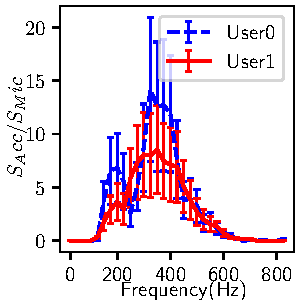
\includegraphics[width=1\textwidth]{chapters/vibvoice/figure/transfer_variance.pdf}
    \caption{Frequency responses of two users' bone-conducted vibrations.}
    %\vspace{-2em}
    \label{fig:vibvoice_bcf}
\end{minipage}
\end{figure}

\noindent\textbf{Frequency Response.}
We further explore the frequency response of bone-conducted vibrations among users. 
Specifically, we measure the frequency response of bone-conducted vibrations as follows: First, we compute the spectrums of audio and vibration data, which is denoted by $S_{Mic}$ and $S_{Acc}$, respectively. Then, we compute the Bone Conduction Function denoted by the frequency response of bone-conducted vibrations by $S_{Acc}/S_{Mic}$ at every frequency band. Fig. \ref{fig:vibvoice_bcf} shows two volunteers' frequency responses, in which the error bars represent the averages and variances.
The acceleration shows higher sensitivity than the microphone within the frequency of $200\text{Hz}\sim500\text{Hz}$, while lower sensitivity at a higher frequency ($>500\text{Hz}$) due to the absorption by the head skull. 
In addition, the frequency response keeps significant similarity among users, indicating the generalization to other users.
Hence, the Bone Conduction Function should consider inter-people diversity and inter-people similarity.

\begin{figure}
\begin{minipage}[t]{0.48\columnwidth}
     \centering
    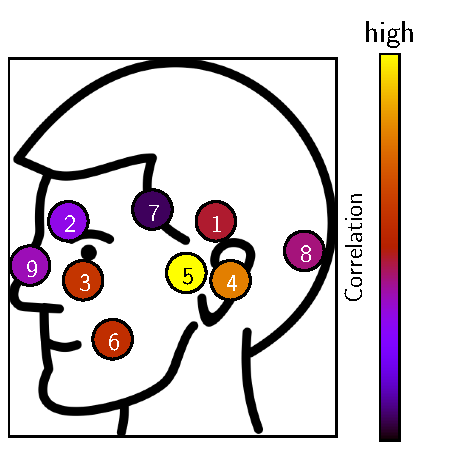
\includegraphics[width=\textwidth]{chapters/vibvoice/figure/correlation.pdf}
    \caption{Intensities of received bone-conducted vibrations on ten locations of the head.}
    \label{fig:vibvoice_head_positison}
\end{minipage}
\hfill
   \begin{minipage}[t]{0.48\columnwidth}
     \centering
    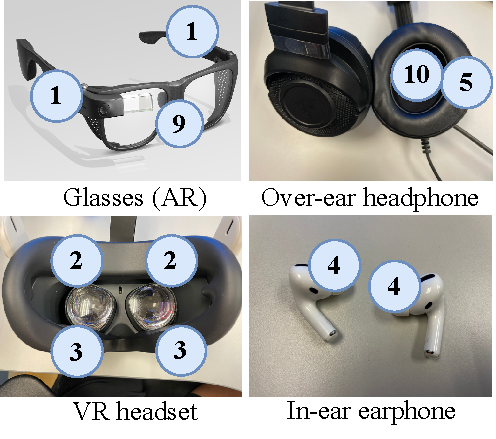
\includegraphics[width=\textwidth]{chapters/vibvoice/figure/devices.pdf}
    \caption{Potential placements on devices.}
    \label{fig:vibvoice_devices}
\end{minipage}
\end{figure}
\noindent\textbf{Locations on the head.}
Bone-conducted vibration exists at various locations on the head. 
As shown in Fig. \ref{fig:vibvoice_head_positison}, we select ten unique locations of interest on the head and measure the intensities of received bone-conducted vibrations. In particular, the nine locations are \#1 \emph{upper ear}, \#2 \emph{eyebrow}, \#3 \emph{cheekbones}, \#4 \emph{ear}, \#5 \emph{temporomandibular joint}, \#6 \emph{cheek}, \#7 \emph{temple}, \#8 \emph{back of the head}, and \#9 \emph{nose}. In addition, we tape EarSense on the interior of the pad of an over-ear headphone, which is denoted as \#10.
Among those positions, some are compatible with commercial HMWs like glasses, headphones, and VR headsets. Fig. \ref{fig:vibvoice_devices} illustrates the corresponding positions on HMWs. The numbers on the HMWs correspond to the locations in Fig. \ref{fig:vibvoice_head_positison}. 
We attach EarSense to the HMWs (when applicable) or on the face for all the following tests. 
We compute Pearson correlation coefficients between the audio and the acceleration on each location and mark the values using a color map in Fig. \ref{fig:vibvoice_head_positison}.
We observe that bone-conducted vibrations exist at most locations of the head. In particular, locations closer to the mouth show higher correlations, indicating a larger possibility of extracting clean speech. 

In summary, our measurements show that bone-conducted vibration has the following characteristics: a) Bone-conducted vibration is robust to environmental voice and only captures the user's speech; b) The user's motion only generates vibrations lower than $85\,\text{Hz}$; c) Bone-conducted vibration has suppressed low and high-frequency audio, which varies across users and within the same user; and d) We can receive audio from multiple locations on the head.

